%==== Document Setup (usthesis)======================================
\documentclass[masters-a,                       %... Document type
               12pt,oneside,openany,a4paper, %... Layout
               a5block,                      %... A5 type block
              afrikaans ,english,           %... Afrikaans default language
               ]{usthesis}
\usepackage[margin=2cm]{geometry}
\usepackage{siunitx}
\usepackage{lipsum} 
\usepackage{graphicx}% http://ctan.org/pkg/graphicx
\usepackage{multirow}% http://ctan.org/pkg/multirow
\usepackage{booktabs}% http://ctan.org/pkg/booktab
\usepackage{amssymb}
\usepackage{subcaption}
%
% PLEASE read the USthesis documentation for the class options
% and how to set line and paragraph spacing
%

%==== Math setup ====================================================
 \usepackage{amsmath}%............................ Advanced math (before fonts)
 %\usepackage{amssymb}%............................ AMS Symbol fonts

%==== Font setup (default is Computer Modern) =======================
 \usepackage[T1]{fontenc}%........................ Type 1 fonts
 \usepackage{textcomp}%........................... Additional text character
 \usepackage{bm}%................................. Bold math symbols (after fonts)

%==== Ref's, Bib's and Nomencl ======================================
 \usepackage{usnomencl}%.......................... List of symbols (in usthesis pack)

 \usepackage{usbib}%.............................. Bibliography    (in usthesis pack)
    \bibliographystyle{usmeg-n}
    \renewcommand\bibfont{\small}
    %% For usmeg-a, the bib is a list of references. If you
    %% are using usmeg-n comment out the following lines

    \renewcommand{\bibname}{References} 

%==== Graphics and Color ============================================
\usepackage{graphicx}%........................... Graphicx loaded in usthesis
\usepackage{color}%.............................. Color setup

%==== Additional USthesis packages ==================================

\usepackage{ussummary}%.......................... Mech Eng summary page (in usthesis pack)

%==== Local Defs ====================================================
\makeatletter


\makeatother
%==== Title Page ====================================================

\title{Report for E-design 344}

\author{Egor Stewdent}
       {Egor Stewdent \\
           123456789\\
           \textcolor{red}{Replace with your own name and number}}

\subject{E-Design 344}
        {}

\ReportDescript{E-Design final report (Assignment \# 1)}

\address{Departement of Electrical and Electronic Engineering,\\
         Universiteit van Stellenbosch,\\
         Privaatsak X1, Matieland 7602.}

%\studyleader{Name of supervisor}

\setdate{9}{2020}

%====================================================================%
%                 T H E   M A I N   D O C U M E N T                  %
%====================================================================%
\begin{document}

\frontmatter%========================================================

\TitlePage
\chapter{Declaration}

By submitting this report electronically, I declare that the entirety of the work contained
therein is my own, original work, that I am the sole author thereof (save to the extent
explicitly otherwise stated), that reproduction and publication thereof by Stellenbosch
University will not infringe any third party rights and that I have not previously in its
entirety or in part submitted it for obtaining any qualifcation.

\vspace{3cm}

\textcolor{red}{ **** Put your signature here and remove this line ****}

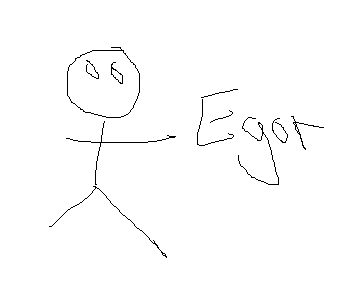
\includegraphics[scale=0.3]{./Figures/Signature.png}\\
\noindent%
\parbox{.5\textwidth}{%
  Signature:\quad\dotfill\par
  \hfill E.\ Stewdent\hspace{1.2cm}\null}


\vspace{1.5cm}
\noindent%
\parbox{.5\textwidth}{%
  Date:\quad\dotfill\par}

\tableofcontents
\listoffigures
\listoftables
\chapter{Nomenclature}
\textcolor{red}{Replace with your own as needed}
\begin{Nomencl}
 \NomGroup{Constants}%-----------------------------------------------
   \item[$\mathrm{g} = $] $\mathrm{9.81\,m/s^2}$

 \NomGroup{Variables}%-----------------------------------------------
   \item[$P$]
                      \UnitLine{Power}{W}



\end{Nomencl}


\endinput


\mainmatter%=========================================================


\chapter{System design}
\section{System overview} \label{sec:system}
Here you insert a block diagram of your voltage regulationa nd signal conditioning system. 
Try to explain \textbf{what} configiation you chose and \textbf{why}. 
There is no need to specify the capacitor and resistor values here, but you want to capture the higher-level functional arrangement you have opted for. The diagram ties together the other chapters in this report and helps the reader understand how you have connected the different funtional blocks together to produce the outputs. For example, a block could be ``Differential amplifier'' or ``level shifting op-amp'' or ``Low-pass filter'' or ``Linear regulator'' and the like. 
Please use a drawing application, such as draw.io, MS Visio, or Power Point and export it as a PDF, so it looks good. If you feel brave, draw them in \LaTeX using Inkscape/\texttt{TikZ}.
Fig.\ \ref{fig:system_diagram} is a bad example that is completely irrelevant and just holds space for your beautiful system diagram. 
\begin{figure}
    \centering
    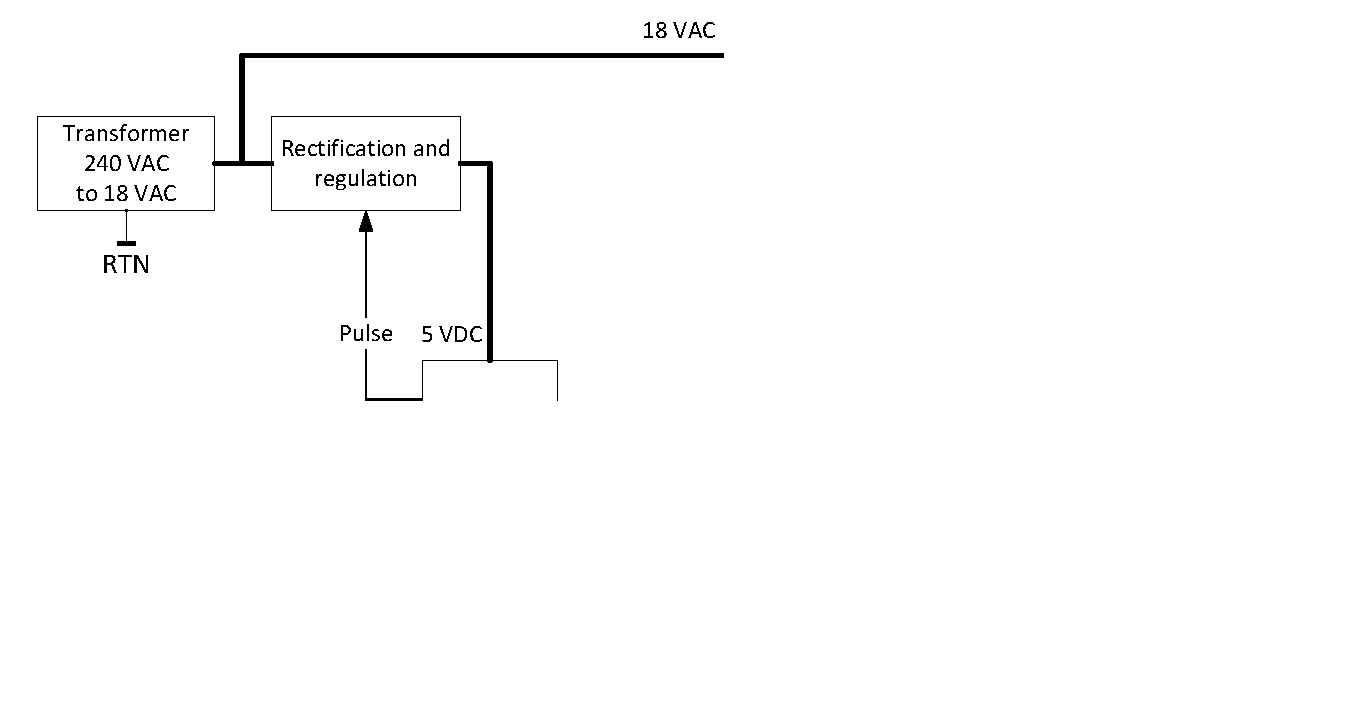
\includegraphics[width = 0.5\linewidth]{Figures/PowerSystemDiagram.pdf}
    \caption{System diagram}
    \label{fig:system_diagram}
\end{figure}

\vfill










\chapter{Voltage regulation}\label{ch:voltage_regulation}
%**********************************************
\section{Background} \label{sec:pwr_backgroud}
%**********************************************
Introduce the reader to what you want to present in this chapter. Include any references to literature you feel is needed. 
In this section, you put a very short summary of infrormation you gatherered from literature (papers, web sites, datasheets) that you used to do the design. Be sure to include the references, which you can add in the \texttt{References.tex} file. 

Some examples of how to cite (all in \texttt{References.bib}): 
It was stated by \cite{Booysen:2013} that ... . Subsequently, he changed his mind and said in  \cite{Gerber:2019} that ... .
While \cite{WebsiteOpAmp} claims it to be ... .

\section{Design} \label{sec:design_rectifier}

In this section, you need to capture your design, which should include the following: 
\begin{itemize}
  \item Design rationale, i.e. what your thinking was behind the design
  \item Design calculations, for example to determine resistor values and capacitor values, or to check for allowed voltage and current ranges and levels. 
  \item Circuit diagram like the one in Figure \ref{fig:circuit_diagram}. I used ``print to PDF'' from LTSpice,  but feel free to use a cropped screengrab if you are PDF-challenged and do not have a PDF printer (there are some free PDF creators online).
\end{itemize}

For your benefit, here is how to write values with units: \SI{150}{\milli\Omega} or \SI{199}{myUnits}, and this is how we write ranges: \numrange{2}{5} \si{\kilo\volt}.

Here is an inline equation $ \frac{55}{45+3}$. Here is a numbered equation in Eq. \ref{eq:myNumberedEquation}.
\begin{equation}
   a = \frac{55}{45+3}
   \label{eq:myNumberedEquation}. 
\end{equation}. 




%**********************************************
\section{Design} \label{sec:pwr_design}
%**********************************************
\begin{figure}
 \footnotesize
   \centering
   \begin{subfigure}[]{0.45\textwidth}
        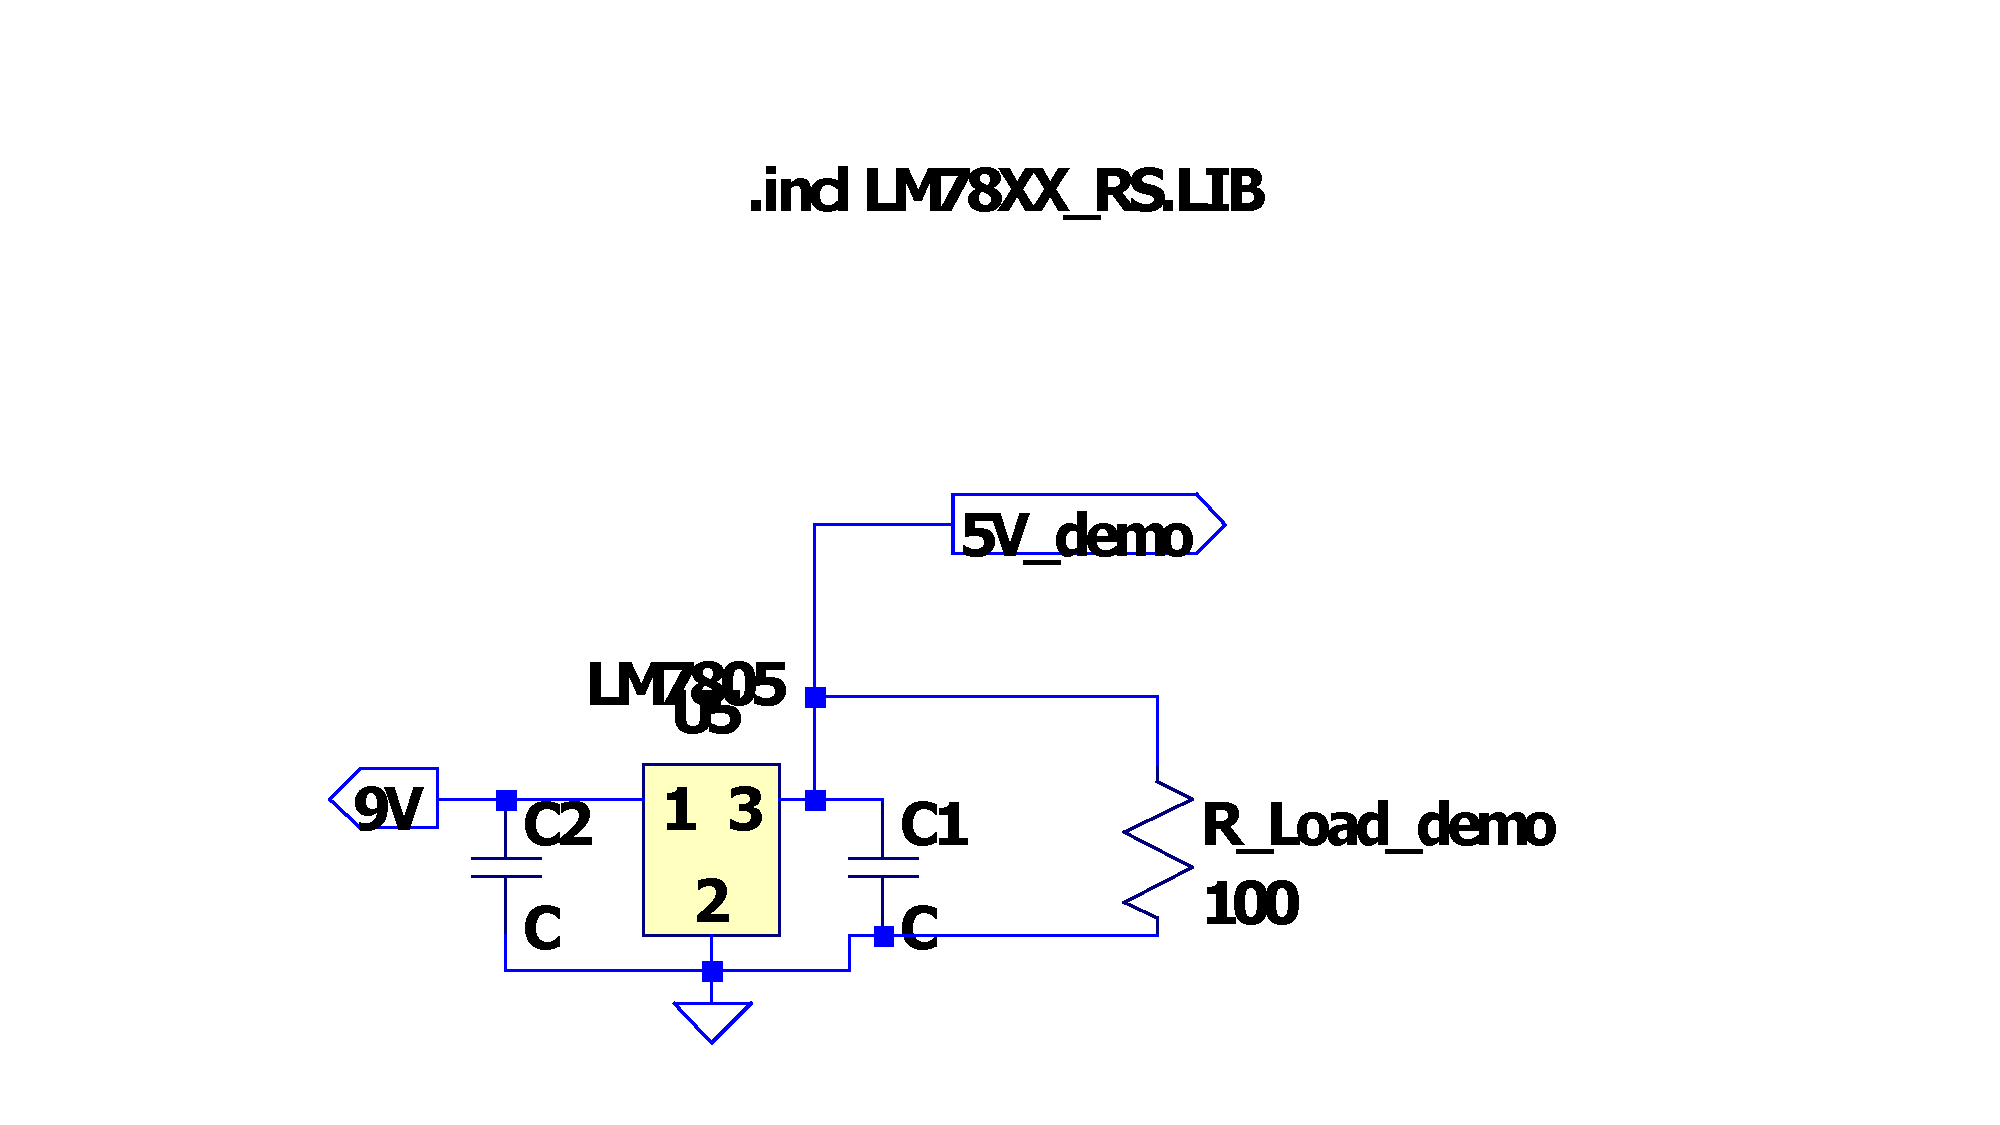
\includegraphics[width=\linewidth]{./Figures/E344_Ass1VoltRegulator_cct}
	  \caption{Linear voltage regulator.} \label{subfig:linear_circuit_diagram}	
   \end{subfigure}
   \begin{subfigure}[]{0.45\textwidth}
  	 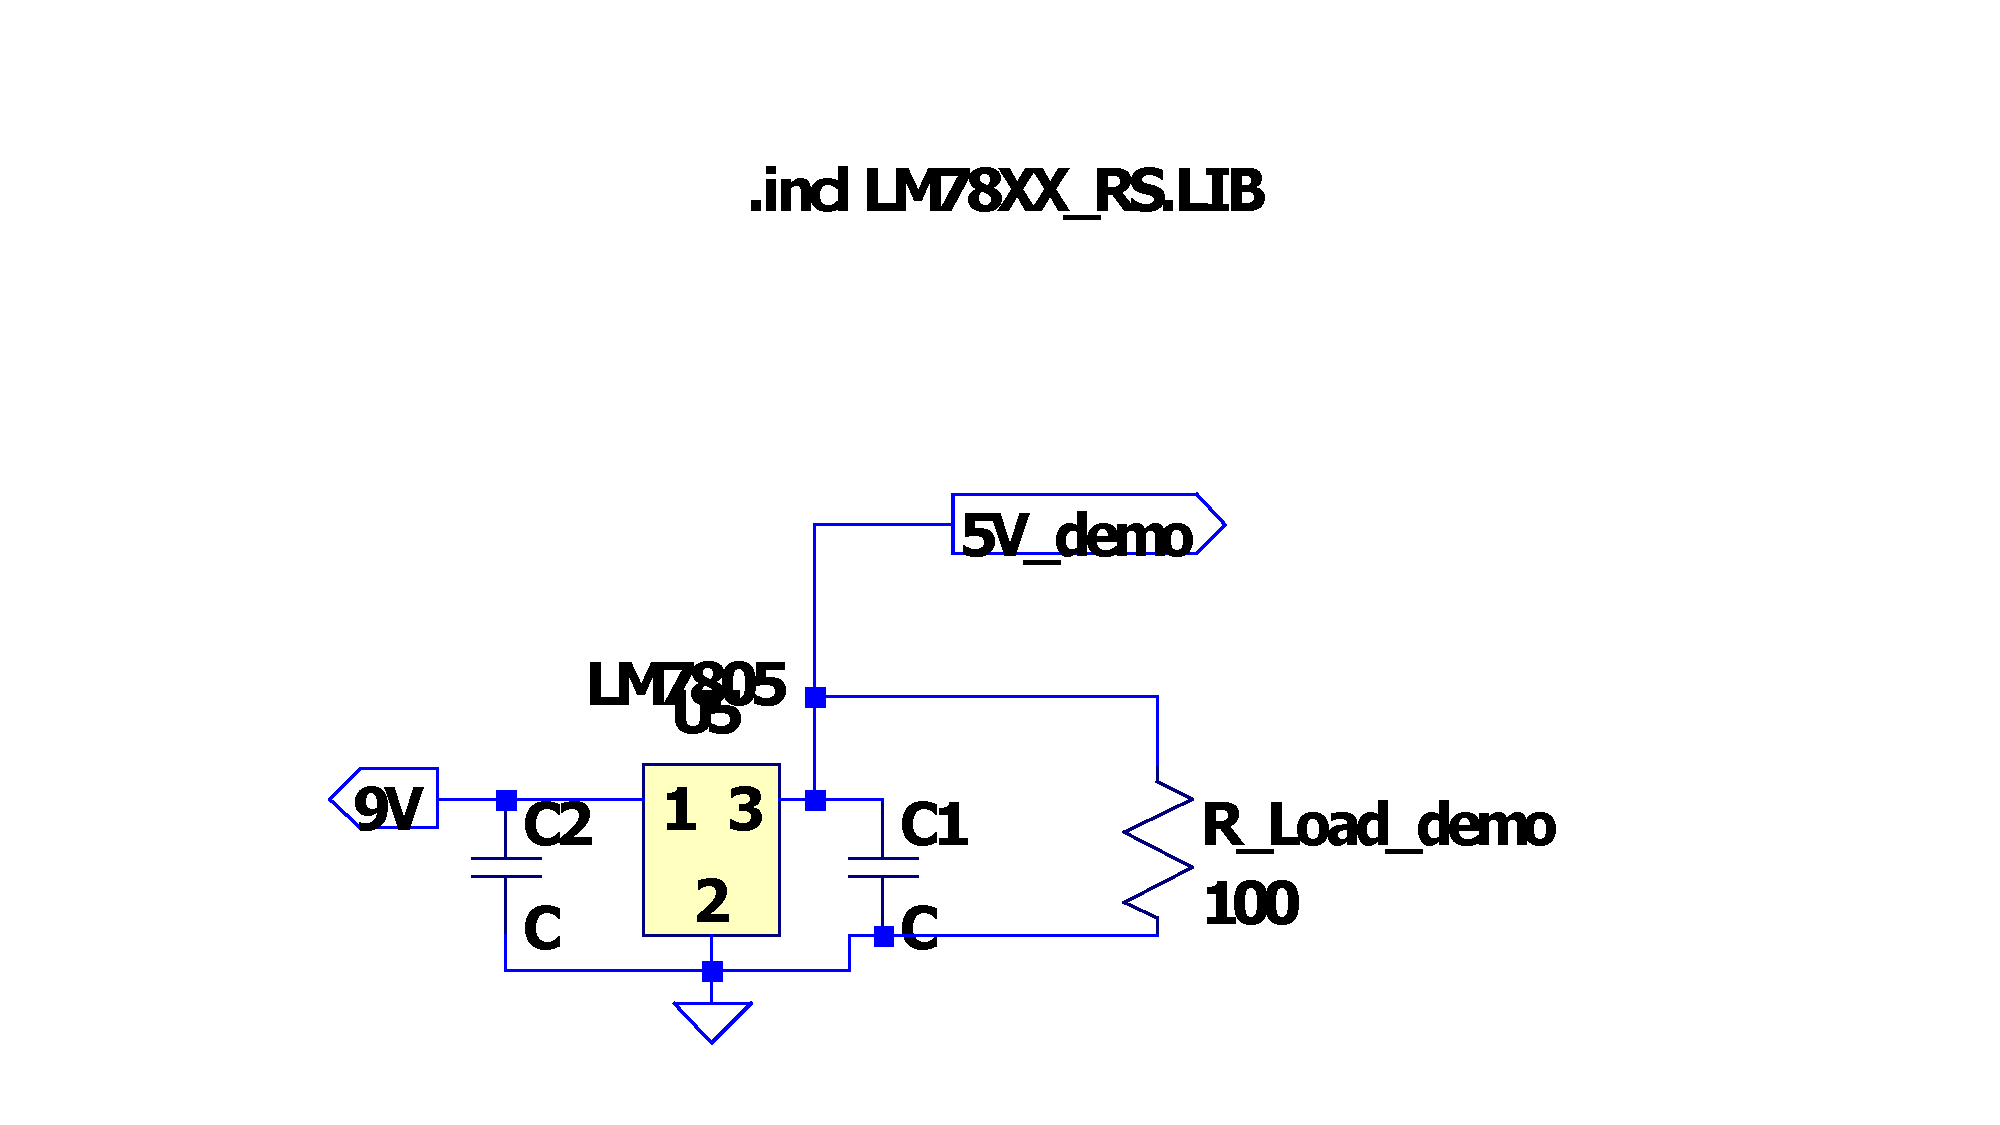
\includegraphics[width=\linewidth]{./Figures/E344_Ass1VoltRegulator_cct}
	  \caption{Switchmode voltage regulator.} \label{subfig:switchmode_circuit_diagram}	
   \end{subfigure}
   \caption {Circuit diagrams of the two voltage regulators}.

      \label{fig:circuit_diagram}
 \end{figure}

In this section, you need to capture your design, which should include the following: 
\begin{itemize}
  \item Design rationale, i.e. what your thinking was behind the design.
  \item References to literature/sources as appropriate \cite{WebsiteOpAmp}. You can assume the reader has an E\&E degree, and will not need trivial explanations or references (e.g. what a resistor is, or what Ohm's law is).   
  \item Analysis of given or expected input conditions. 
  \item Design calculations, for example to determine resistor values and capacitor values, or to check for allowed voltage and current ranges and levels. 
  \item Expected values and ranges based on your design. 
  \item Schematic circuit diagram, like in Figure \ref{subfig:switchmode_circuit_diagram} (which is, again, just an irrelevant example). 
  \item Explain your choice of supply buy referring to the advantages and disadvantages of each. 
\end{itemize}

%**********************************************
\section{Simulation} \label{sec:pwr_simu}
%**********************************************


\begin{figure}
 \footnotesize
 \centering
    \begin{subfigure}[]{0.55\textwidth}
              \centering
  		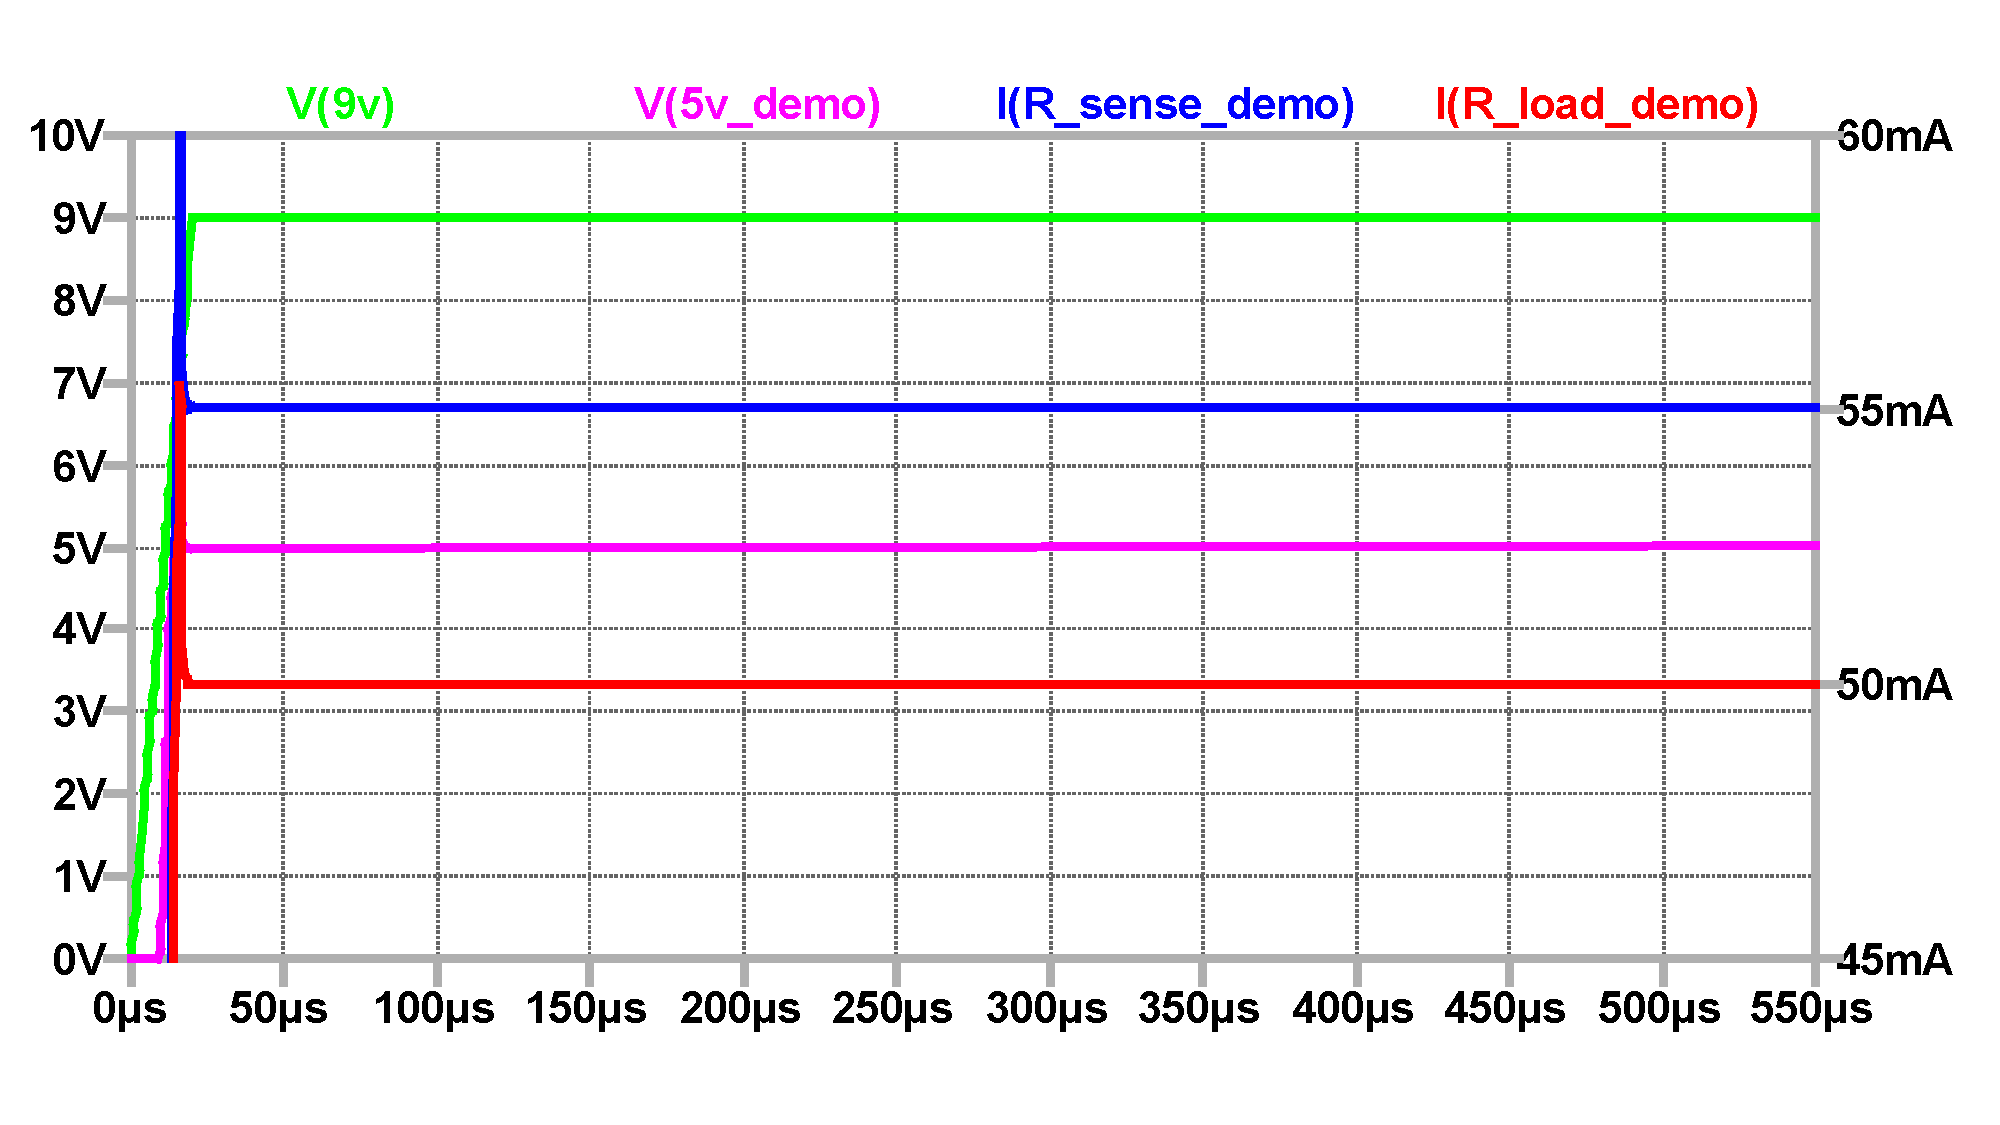
\includegraphics[width=1\linewidth]{./Figures/E344_VoltRegulator.pdf}
		    \caption{} \label{subfig:pwr_simu_rect}
     \end{subfigure}
     \begin{subfigure}[]{0.4\textwidth}
             \centering
  		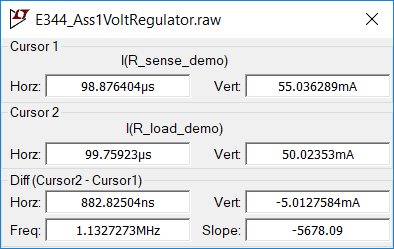
\includegraphics[width=1.0\linewidth]{./Figures/Screengrab2}
		   \caption{ } \label{subfig:pwr_meas_rect}
     \end{subfigure}
    \begin{subfigure}[]{0.55\textwidth}
              \centering
  		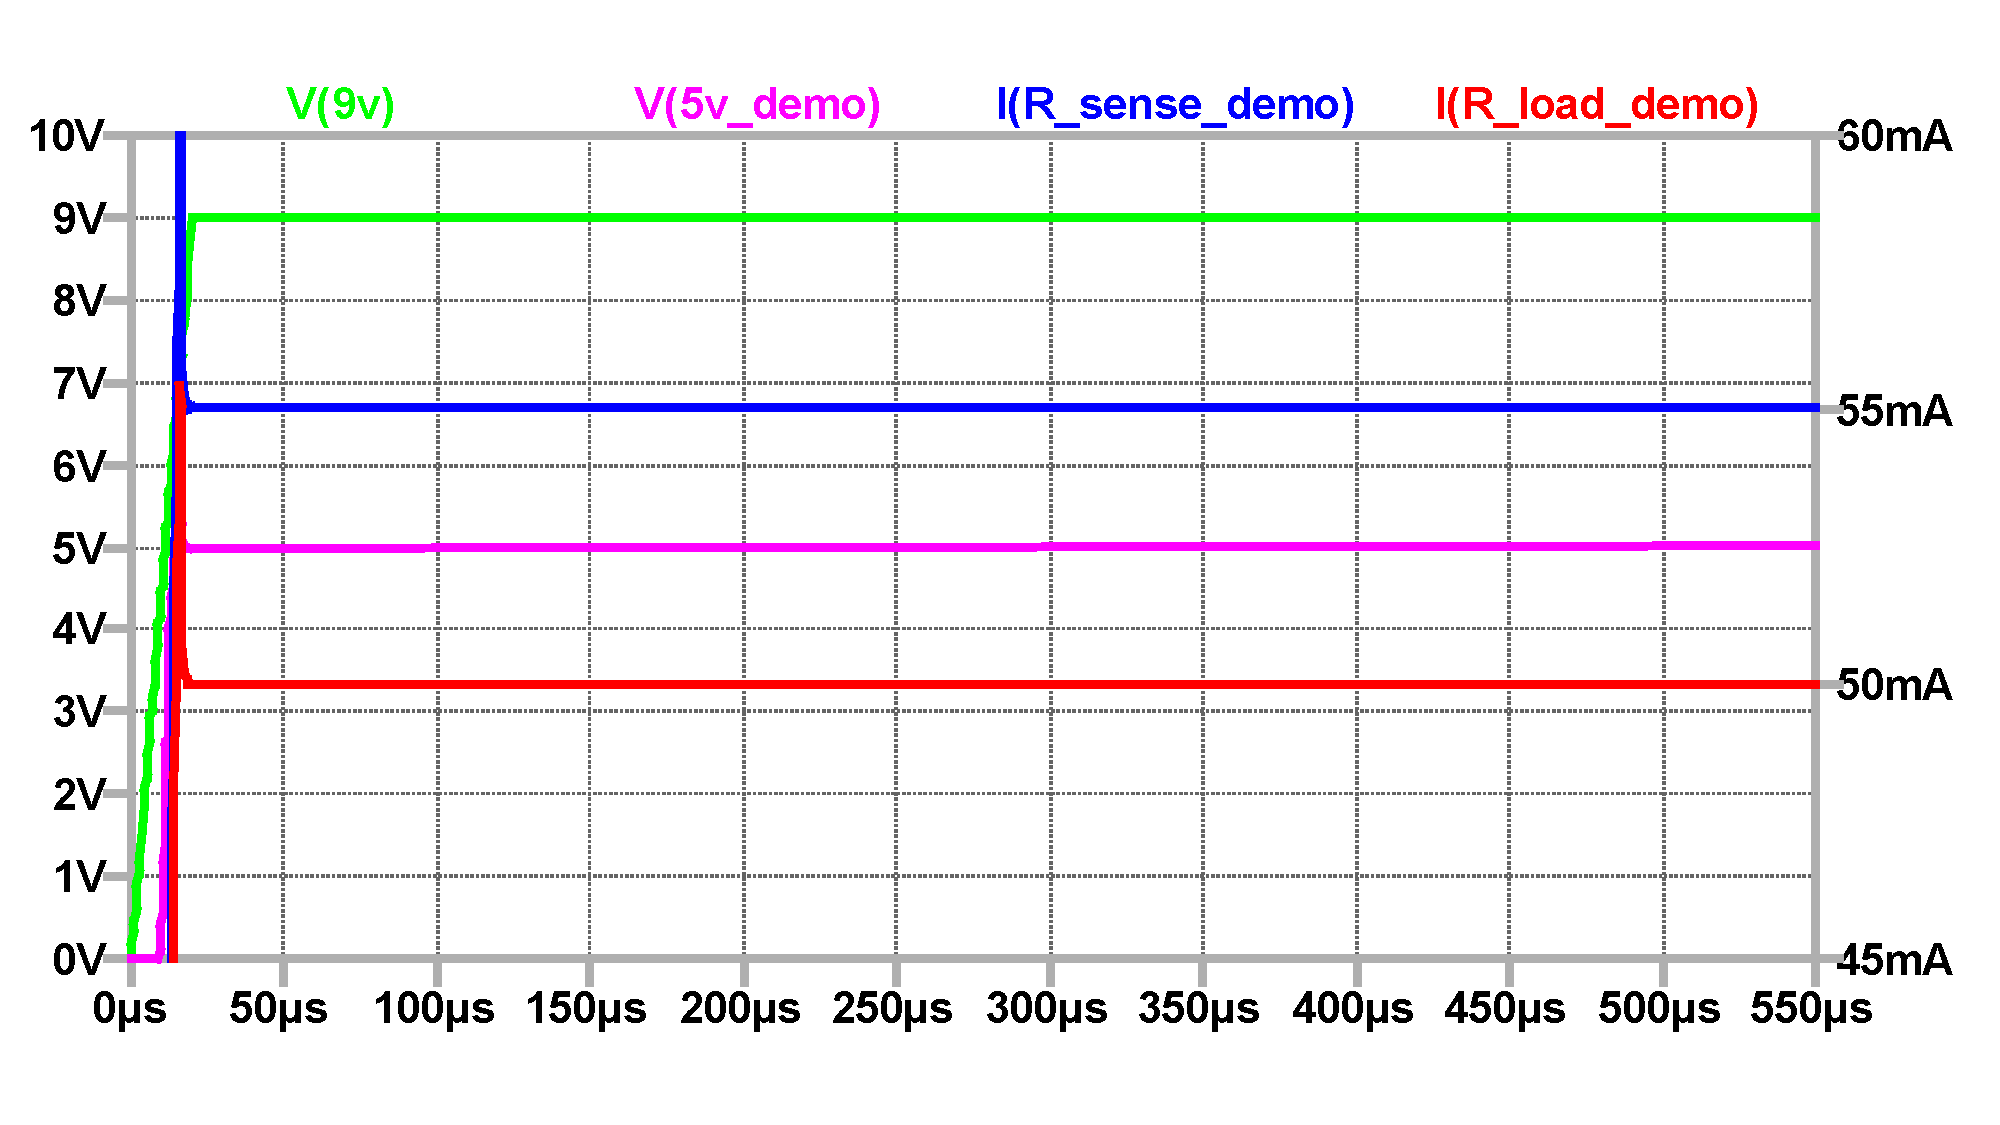
\includegraphics[width=1\linewidth]{./Figures/E344_VoltRegulator.pdf}
		    \caption{} \label{subfig:pwr_simu_rect}
     \end{subfigure}
    \begin{subfigure}[]{0.4\textwidth}
              \centering
  		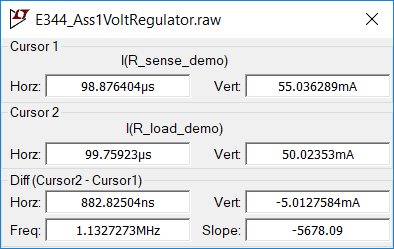
\includegraphics[width=1\linewidth]{./Figures/Screengrab2}
		    \caption{} \label{subfig:pwr_simu_rect}
     \end{subfigure}
   \caption[\textcolor{red}{I am the short caption that appears in the List of Figures list, without references}]{Voltage regulation, comparing the linear and switchmode regulators... (a)  Blah blah. (b)  Blah blah.  (c)  Blah blah. (d) Blah blah.   Based on the datasheet of XXXX in \cite{WebsiteOpAmp}}
    \label{fig:simulation_results_box}
 \end{figure}

In this section, you want to demonstrate, by means of referring to simulation results, using the designed circuit, how your circuit is expected to behave. Present and report on your simulated results in Figure \ref{fig:simulation_results_box} Be absolutely sure that the text and information in your report are readable. 

You can use screengrabs or photos of the oscilloscope, or download the CSVs and plot them as PDFs using Matlab, Excel or similar. 
You can also use tables, example of which are presented in Tables \ref{tab:table1} and \ref{tab:table2}.


\begin{table}
        \centering
        \footnotesize
        \caption{Example of a table.}
         \begin{tabular}{c@{\qquad}rrrr}
          \toprule
             & 2017 & 2018 & $\Delta_{Abs}$ & $\Delta_{DiD}$\\
          \midrule
          A & 9,868      & 10,399 & +5 & -11\\
          B & 10,191     & 10,590 & +4 & -12\\
          \bottomrule
        \end{tabular}
     \label{tab:table1}
\end{table}


\begin{table}
         \centering
        \footnotesize
        \caption{Example of another table.}

         \begin{tabular}{c@{\qquad}rrrr}
          \toprule
          \multirow{2}{*}{\raisebox{-\heavyrulewidth}{Schools }} & \multicolumn{2}{c}{Total energy used}& \multicolumn{2}{c}{Change}\\
          \cmidrule{2-5}
            & 2017 & 2018 & $\Delta_{Abs}$ & $\Delta_{DiD}$\\
            & [kWh] & [kWh] & [\%] & [\%] \\
          \midrule
          A & 9,868      & 10,399 & +5 & -11\\
          B & 10,191     & 10,590 & +4 & -12\\
          \bottomrule
        \end{tabular}
     \label{tab:table2}
\end{table}


%**********************************************
\section{Summary and implementation}
%**********************************************
State whether your design performs as expected and what the limitations are or things to keep in mind are. 



\chapter{System and conclusion}
\vspace{-5mm}
\section{System}
% Report on the ``so what'' or the take-away of the ciruit you designed in this report.  
% Report on noise levels and how the Heart rate sensor will fit into the system (E.g. what the calibration will look like and what the the measurement error will be given the range, quantisation error and noise). 
The circuit works as expected. This Heart Rate Sensor conditioning circuit will fit nicely into the system. The MCU can easily read the pulse inputs and count every high pulse for a duration of time and then relate that to BPM. This will only need one pin from the MCU, while also using very little current. The circuit is effective and make accurate pulses. In the way the circuit is built, it also allows it to be used with any DC offest from the heart beat sensor, given that it is between the ranges of \numrange{0}{5} \si{\volt}.\par
It is not a very difficult circuit to implement, except when one wants to introduce a transducer to convert frequency signals to an analog output. It is quite difficult to find proper sources for this implantation online, let alone in stander Engineering textbooks. Once a source is found however, it can be even more difficult given \texttt{LTSpice} struggles with timestep errors.


\section{Lessons learnt}
% Write down at least three of the most important things you have learnt in Assignment 2, and state what you would have done differently if you had another chance. 
Things that I learned in assignment 2:
\begin{itemize}
    \item Most importantly, I feel much more confident in my knowledge of \LaTeX and \texttt{LTSpice} and have learned hwo to use them properly, while also finding out how they are limited in certain aspects.
    \item I learned how to implement filters in a more effective way,a nd how differnet filters can be used for different use cases.
    \item I learned that you can build a lot of simple components like One-Shot timers, comparators, transducers and filters only by using op-amps, resistors and capacitors.
    \item I learned that it is always wiser to start early and not procrastinate. Also, write down while you are designing so that you can always backtrack and find your steps. 
\end{itemize}

\par
If I had another chance, I would spend more time working on the transducer. I spent almost 20 hours, if not more, on that part of the designed, but still could not get it working. I decided not to do it when I realised that if I keep working on this one part of the design, I will never finish on time.

\chapter{System and conclusion}
\vspace{-5mm}
\section{System}


\section{Lessons learnt}
Write down at least three of the most important things you have learned or lessons you acquired from Assignment 1.


\appendix%===========================================================


\backmatter%=========================================================

\bibliography{References}
\renewcommand{\thesection}{A.\arabic{section}}
\renewcommand{\thechapter}{A.}
\begin{appendix}

     \chapter{Appendix A: Social contract}
     \vspace{-15mm}
     \begin{figure}[!htb]
     \centering
     	\fbox{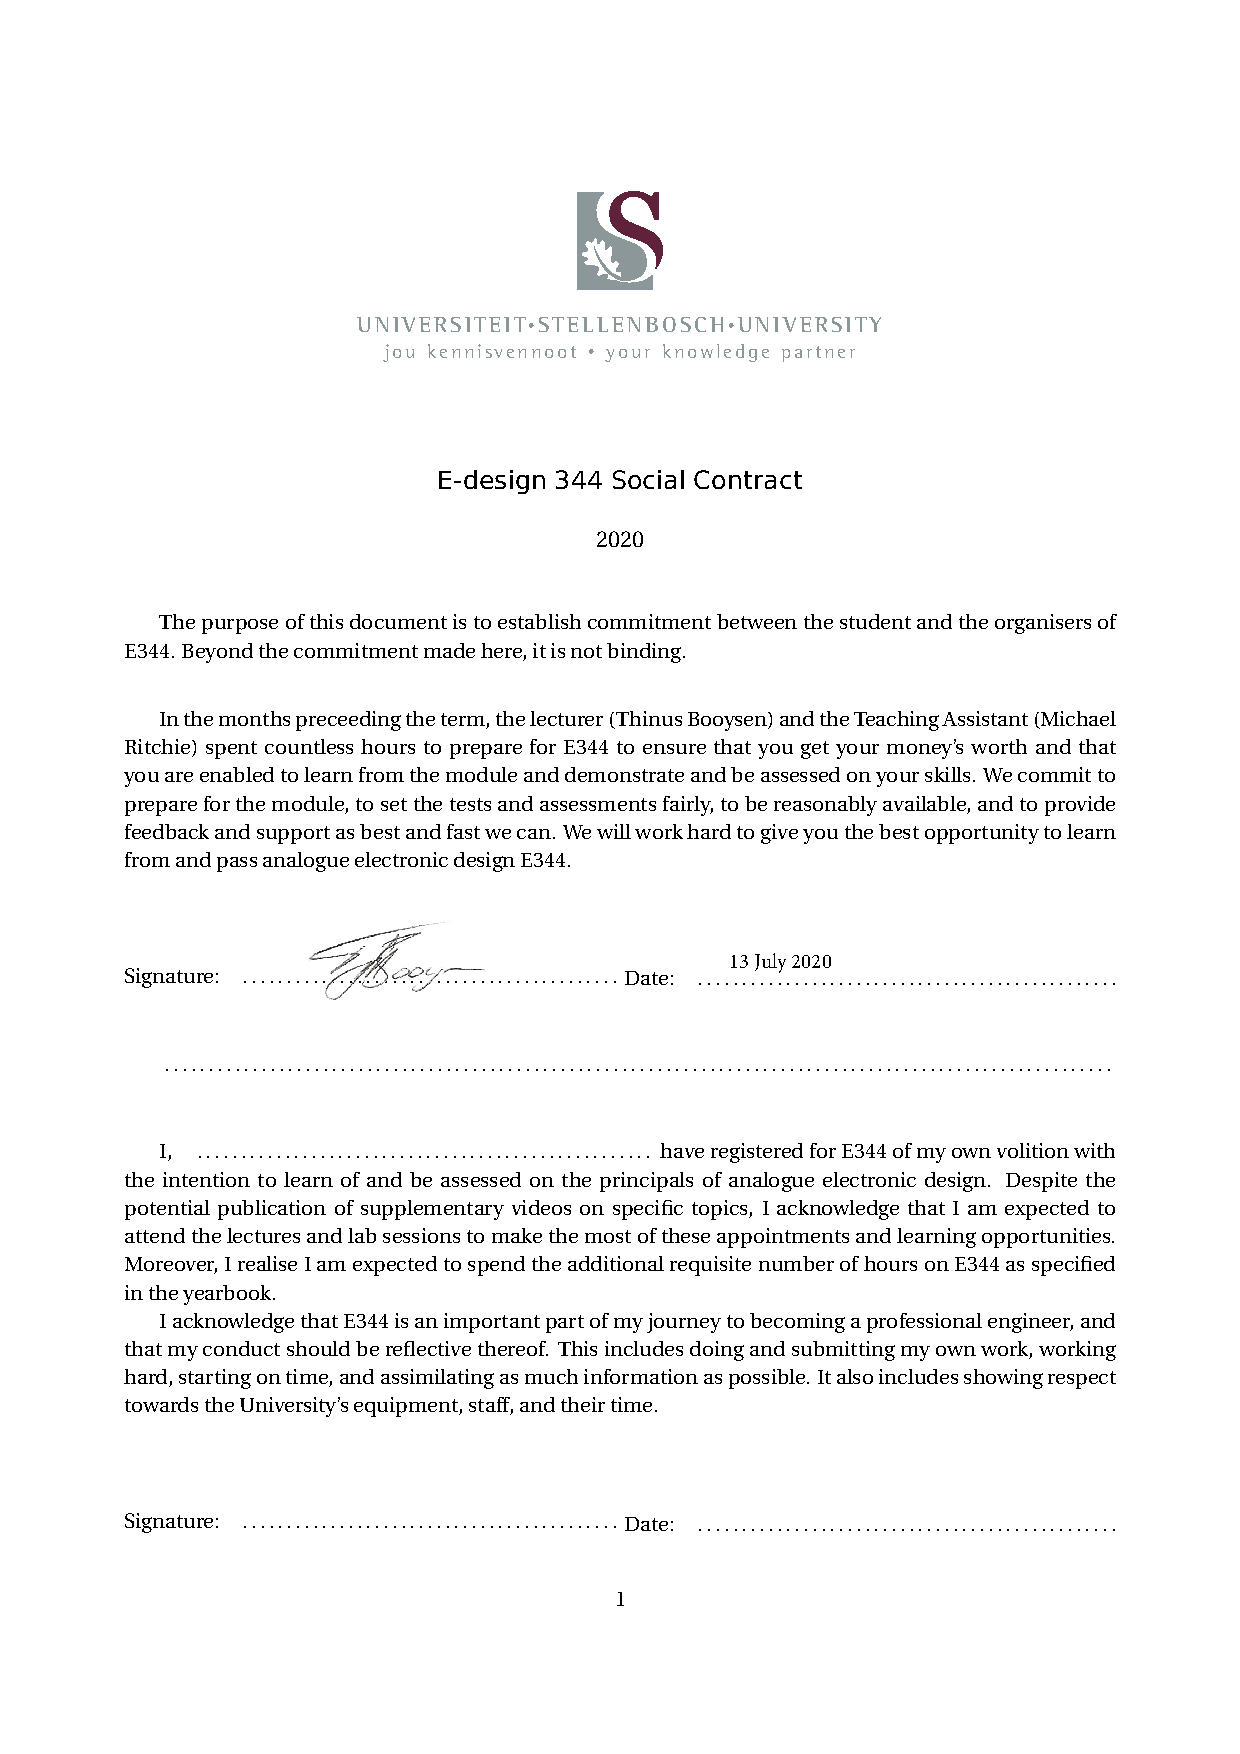
\includegraphics[width=0.78\linewidth]{./Figures/SocialContract.pdf}}
       \label{fig:social_contract}
	\end{figure}
\chapter{GitHub Activity Heatmap}
\makeatletter\@mkboth{}{Appendix}\makeatother
\label{appen:github_heatmap}
\textcolor{red}{Take a screenshot of your github version control activity heatmap and insert here. }

     \begin{figure}[!htb]
     \centering
     	\fbox{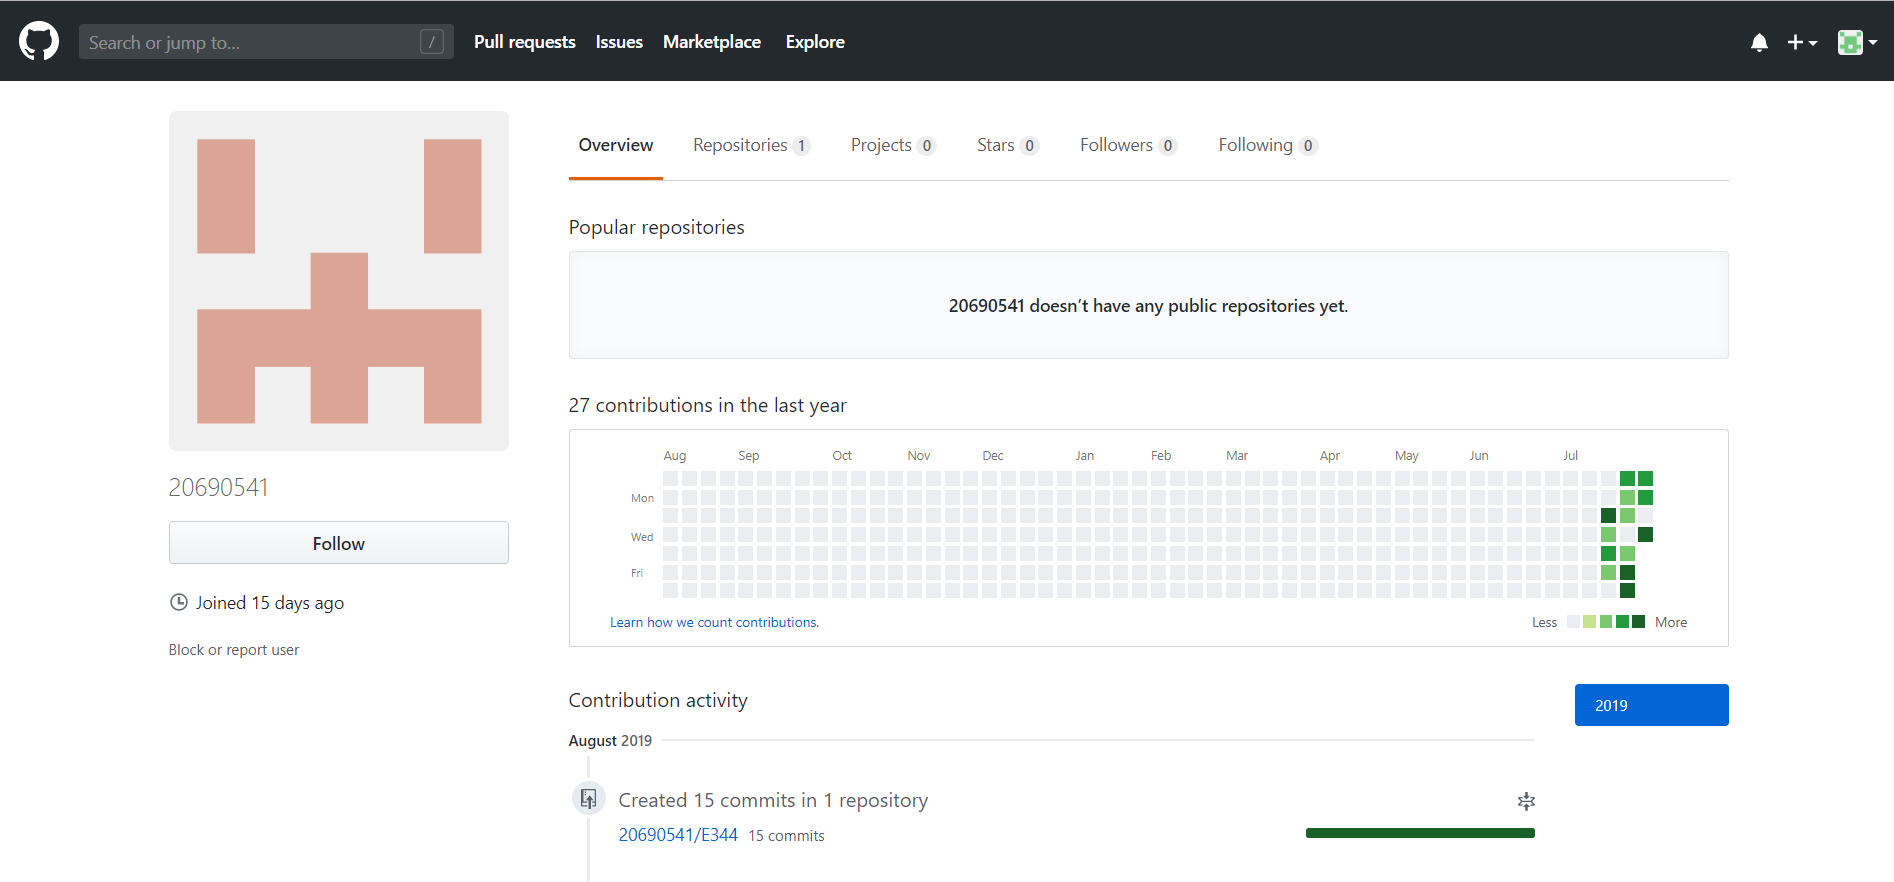
\includegraphics[width=1\linewidth]{./Figures/GitHub.png}}
	\label{fig:github}
	\end{figure}
     \chapter{Stuff you want to include}

\lipsum
\end{appendix}
\end{document}
